% Created 2025-04-29 Tue 19:47
% Intended LaTeX compiler: pdflatex
\documentclass[11pt]{article}
\usepackage[utf8]{inputenc}
\usepackage[T1]{fontenc}
\usepackage{graphicx}
\usepackage{longtable}
\usepackage{wrapfig}
\usepackage{rotating}
\usepackage[normalem]{ulem}
\usepackage{amsmath}
\usepackage{amssymb}
\usepackage{capt-of}
\usepackage{hyperref}
\usepackage{minted}
\author{Hankertrix}
\date{\today}
\title{Math Module 5A Notes}
\hypersetup{
 pdfauthor={Hankertrix},
 pdftitle={Math Module 5A Notes},
 pdfkeywords={},
 pdfsubject={},
 pdfcreator={Emacs 30.1 (Org mode 9.7.11)}, 
 pdflang={English}}
\begin{document}

\maketitle
\setcounter{tocdepth}{2}
\tableofcontents \clearpage\section{Definitions}
\label{sec:orgc9a1f46}

\subsection{Vectors in \(\mathbb{R}^n\)}
\label{sec:org3c2a67e}
Let \(n\) be a positive integer.


We define \(\mathbb{R}^n\) to be the set of all ordered \(n\)-tuples of elements from \(\mathbb{R}\), i.e:
\[\mathbb{R}^n = \{(x_1, x_2, \ldots, x_n): x_1, x_2, \ldots, x_n \in \mathbb{R}\}\]

An element \(\boldsymbol{x} = (x_1, x_2, \ldots, x_n) \in \mathbb{R}^n\) is called a \textbf{vector}. We usually use boldface symbols to denote vectors.


A vector is ordered, i.e:
\[(1, 2, 5) \ne (1, 5, 2)\]

Repetitions also matter:
\[(1, 1, 2) \ne (1, 2)\]
\subsubsection{Example}
\label{sec:org6e8f0ed}
\[\boldsymbol{x} = (-1, \pi, \sin 2, \frac{1}{2}, 1000) \text{ is a vector in } \mathbb{R}^5\]
\subsection{Geometric interpretation of \(\mathbb{R}^2\) or \(\mathbb{R}^3\)}
\label{sec:org75e6633}
\begin{itemize}
\item A vector in \(\mathbb{R}^2 \text{ or } \mathbb{R}^3\) has length and direction, illustrated with an arrow.
\item We use \(\overrightarrow{P_1 P_2}\) for the vector from \(P_1\) to \(P_2\).
\item With \(P_1 = (x_1, y_1, z_1), P_2 = (x_2, y_2, z_2)\), we have:
\end{itemize}
\[\overrightarrow{P_1 P_2} = (x_2 - x_1, y_2 - y_1, z_2 - z_1)\]

In particular, with \(O = (0, 0, 0), P = (x, y, z)\), we get:
\[\overrightarrow{OP} = (x, y, z)\]
\subsection{Scalars}
\label{sec:org7216f77}
Scalars are basically real numbers. For example, 1.2 and \(\pi\) are scalars.
\subsection{Zero vector}
\label{sec:org322575d}
The zero vector in \(\mathbb{R}^n\) is the vector:
\[\boldsymbol{0} = (0, 0, \ldots, 0)\]
\subsection{Negative vectors}
\label{sec:org1ccf3b4}
For \(\boldsymbol{x} = (x_1, x_2, \ldots, x_n) \in \mathbb{R}^n\), its \textbf{additive inverse} (or \textbf{negative}) is denoted by \(- \boldsymbol{x}\) and is given by:
\[- \boldsymbol{x} = (-1) \boldsymbol{x} = (-x_1, -x_2, \ldots, -x_n)\]
\subsection{Sum of vectors}
\label{sec:orgd7676fd}
Let \(\boldsymbol{x} = (x_1, x_2, \ldots, x_n) \text{ and } \boldsymbol{y} = (y_1, y_2, \ldots, y_n)\) be vectors in \(\mathbb{R}^n\). The sum is defined as follows:
\[\boldsymbol{x} + \boldsymbol{y} = (x_1 + y_1, x_2 + y_2, \ldots, x_n + y_n)\]
\subsection{Difference of vectors}
\label{sec:org220ae69}
The difference \(\boldsymbol{x} - \boldsymbol{y}\) of \(\boldsymbol{x}, \boldsymbol{y} \in \mathbb{R}^n\) is defined as:
\[\boldsymbol{x} - \boldsymbol{y} = \boldsymbol{x} + (- \boldsymbol{y})\]
\subsection{Product of a vector and a scalar}
\label{sec:org28eed28}
Let \(\boldsymbol{x} = (x_1, x_2, \ldots, x_n) \text{ and } \boldsymbol{y} = (y_1, y_2, \ldots, y_n)\) be vectors in \(\mathbb{R}^n\) and let \(c\) be a scalar. The product is defined as follows:
\[c \boldsymbol{x} = (cx_1, cx_2, \ldots, cx_n)\]

\newpage
\subsection{Dot product of vectors (Scalar product or Euclidean inner product)}
\label{sec:orga1e603d}
For:
\[\boldsymbol{x} = (x_1, x_2, \ldots, x_n) \in \mathbb{R}^n, \boldsymbol{y} = (y_1, y_2, \ldots, y_n) \in \mathbb{R}^n\]

Their scalar product (or Euclidean inner product, or dot product) \(\boldsymbol{x} \cdot \boldsymbol{y}\), is defined as:
\[\boldsymbol{x} \cdot \boldsymbol{y} = x_1 y_1 + x_2 y_2 + \cdots + x_n y_n = \sum_{i = 1}^n x_i y_i\]

Note that \(\boldsymbol{x} \cdot \boldsymbol{y}\) is a scalar, not a vector.
\subsubsection{Example:}
\label{sec:orgfe6f06e}
With \(\boldsymbol{x} = (1, 2, 3, 4), \boldsymbol{y} = (-2, 3, -1, 1)\), we have:
\begin{align*}
\boldsymbol{x} \cdot \boldsymbol{y} &= 1 \cdot (-2) + 2 \cdot 3 + 3 \cdot (-1) + 4 \cdot 1 \\
&= 5
\end{align*}
\subsection{Norm of a vector}
\label{sec:orge5e40f3}
The norm \(||\boldsymbol{x}||\) of a vector \(\boldsymbol{x}\) in \(\mathbb{R}^n\) is defined by:
\[||\boldsymbol{x}|| = \sqrt{\boldsymbol{x} \cdot \boldsymbol{x}}\]
\subsubsection{Example}
\label{sec:orgf51b8ad}
The normal of the vector \(\boldsymbol{x} = (1, 0, 3, -2)\) in \(\mathbb{R}^4\) is:
\begin{align*}
||\boldsymbol{x}|| &= \sqrt{\boldsymbol{x} \cdot \boldsymbol{x}} \\
&= \sqrt{1^2 + 0^2 + 3^2 + (-2)^2} \\
&= \sqrt{14}
\end{align*}
\subsection{Geometric view of the dot product}
\label{sec:org017bfa5}
Let \(\boldsymbol{x}\) and \(\boldsymbol{y}\) be two vectors in \(\mathbb{R}^2\) or \(\mathbb{R}^3\), and let \(\theta\) be the angle between \(\boldsymbol{x}\) and \(\boldsymbol{y}\), where \(\theta \in [0, \pi]\). Then:
\[\boldsymbol{x} \cdot \boldsymbol{y} = || \boldsymbol{x} || \cdot || \boldsymbol{y} || \cos \theta\]

Since \(\theta \in [0, \pi]\), it follows that:
\[\theta = \arccos \left( \frac{\boldsymbol{x} \cdot \boldsymbol{y}}{|| \boldsymbol{x} || \cdot || \boldsymbol{y} ||} \right)\]
\subsection{Cauchy-Schwarz inequality}
\label{sec:org74fe536}
Note that for \(\boldsymbol{x}, \boldsymbol{y} \in \mathbb{R}^2\) or \(\boldsymbol{x}, \boldsymbol{y} \in \mathbb{R}^3\), we have:
\begin{align*}
| \boldsymbol{x} \cdot \boldsymbol{y} | &= || \boldsymbol{x} || \cdot || \boldsymbol{y} || \cdot | \cos \theta | \\
&\le || \boldsymbol{x} || \cdot || \boldsymbol{y} || \quad (\because | \cos \theta | \le 1 \text{ when } 0 \le \theta \le \pi)
\end{align*}

Hence, let \(\boldsymbol{x}\) and \(\boldsymbol{y}\) be vectors in \(\mathbb{R}^n\). Then:
\[| \boldsymbol{x} \cdot \boldsymbol{y} | \le || \boldsymbol{x} || \cdot || \boldsymbol{y} ||\]
\subsection{Triangle inequality}
\label{sec:orgcc153bf}
Let \(\boldsymbol{x}\) and \(\boldsymbol{y}\) be vectors in \(\mathbb{R}^n\), then:
\[|| \boldsymbol{x} + \boldsymbol{y} || \le || \boldsymbol{x} || + || \boldsymbol{y} ||\]
\subsection{Orthogonality}
\label{sec:orgdf52c01}
Two vectors \(\boldsymbol{x} \text{ and } \boldsymbol{y}\) in \(\mathbb{R}^n\) are said to be orthogonal if \(\boldsymbol{x} \cdot \boldsymbol{y} = 0\).


\begin{itemize}
\item In \(\mathbb{R}^2\) or \(\mathbb{R}^3\), two non-zero vectors are perpendicular if and only if they are orthogonal. It is useful to think about orthogonal vectors in higher dimensions in the same way, even if it makes no geometrical sense.
\item Since \(\boldsymbol{0} \cdot \boldsymbol{x} = 0\), the zero vector is orthogonal to all vectors.
\end{itemize}
\subsubsection{Example}
\label{sec:org5244279}
The vectors \(\boldsymbol{x} = (1, 2, 1, 2)\) and \(\boldsymbol{y} = (3, 3, -3, -3)\) are orthogonal vectors in \(\mathbb{R}^4\), since:
\begin{align*}
\boldsymbol{x} \cdot \boldsymbol{y} &= 1 \cdot 3 + 2 \cdot 3 + 1 \cdot (-3) + 2 \cdot (-3) \\
&= 0
\end{align*}
\subsection{Pythagoras' theorem in \(\mathbb{R}^n\)}
\label{sec:org38f7552}
If \(\boldsymbol{x}\) and \(\boldsymbol{y}\) are orthogonal vectors in \(\mathbb{R}^n\), then:
\[|| \boldsymbol{x} + \boldsymbol{y} ||^2 = || \boldsymbol{x} ||^2 + || \boldsymbol{y} ||^2\]
\subsection{Projections in \(\mathbb{R}^n\)}
\label{sec:org4732599}
Suppose \(\boldsymbol{x}, \boldsymbol{a} \in \mathbb{R}^n, \boldsymbol{a} \ne 0\).


There exist \textbf{unique} \(\boldsymbol{x}_1, \boldsymbol{x}_2 \in \mathbb{R}^n\) such that:
\[\boldsymbol{x} = \boldsymbol{x}_1 + \boldsymbol{x}_2, \quad \boldsymbol{x}_1 = k \boldsymbol{a}, l \in \mathbb{R}, \quad \text{and } \boldsymbol{x}_2 \cdot \boldsymbol{a} = 0\]

This unique representation is given by:
\[\boldsymbol{x}_1 = \frac{\boldsymbol{x} \cdot \boldsymbol{a}}{|| \boldsymbol{a} ||^2} \boldsymbol{a}, \quad \boldsymbol{x}_2 = \boldsymbol{x} - \frac{\boldsymbol{x} \cdot \boldsymbol{a}}{|| \boldsymbol{a} ||^2} \boldsymbol{a}\]

\(\boldsymbol{x}_1\) is called the \textbf{orthogonal projection} of \(\boldsymbol{x}\) onto \(\boldsymbol{a}\) and is denoted \(proj_a \boldsymbol{x}\).
\subsection{Cross product of vectors}
\label{sec:orgb3d46fd}
Consider \(\boldsymbol{x} = (x_1, x_2, x_3), \boldsymbol{y} = (y_1, y_2, y_3)\) in \(\mathbb{R}^3\).


The \textbf{cross product} \(\boldsymbol{x} \times \boldsymbol{y}\) of \(\boldsymbol{x}\) and \(\boldsymbol{y}\) is:
\[\boldsymbol{x} \times \boldsymbol{y} = (x_2 y_3 - x_3 y_2, -x_1 y_3 + x_3 y_1, x_1 y_2 - x_2 y_1) \in \mathbb{R}^3\]

To remember the formula above, let:
\[\boldsymbol{i} = (1, 0, 0), \quad \boldsymbol{j} = (0, 1, 0), \quad \boldsymbol{k} = (0, 0, 1)\]

And use this scheme:

\begin{center}
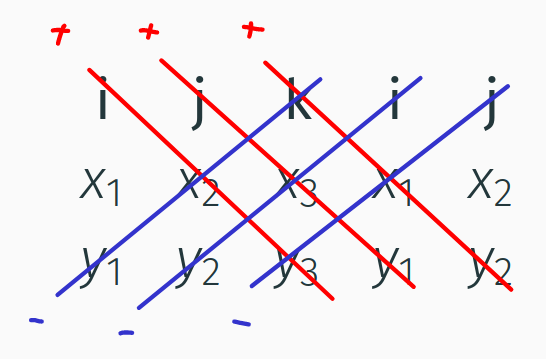
\includegraphics[scale=1.0]{./images/cross-product.png}
\end{center}
\begin{align*}
&x_2 y_3 \boldsymbol{i} + x_3 y_1 \boldsymbol{j} + x_1 y_2 \boldsymbol{k} - x_2 y_1 \boldsymbol{k} - x_3 y_2 \boldsymbol{i} - x_1 y_3 \boldsymbol{j} \\
&= (x_2 y_3 - x_3 y_2) \boldsymbol{i} + (x_3 y_1 - x_1 y_3) \boldsymbol{j} + (x_1 y_2 - x_2 y_ 1) \boldsymbol{k}
\end{align*}
\subsection{Planes}
\label{sec:orgf92d58b}
With a \textbf{normal vector} to a plane in \(\mathbb{R}^3\), we mean a non-zero vector that is perpendicular to the plane.


Suppose the plane \(\Pi\) contains the point \(P_0 = (x_0, y_0, z_0)\) and has normal vector \(\boldsymbol{n} = (a, b, c)\). We see that a point \(P = (x, y, z)\) lies in \(\Pi\) if and only if \(\overrightarrow{P_0P}\) is orthogonal to \(\boldsymbol{n}\).
\subsubsection{Equations for a plane}
\label{sec:org96a217d}
\begin{center}
\(P = (x, y, z)\) lies in the plane \(\Pi\)
\[\Updownarrow\]
\(\overrightarrow{P_0 P}\) is orthogonal to \(\boldsymbol{n}\)
\[\Updownarrow\]
\[\boldsymbol{n} \cdot \overrightarrow{P_0 P} = 0\]
\[\Updownarrow\]
\[a(x - x_0) + b(y - y_0) + c(z - z_0) = 0\]
\[\Updownarrow\]
\[ax + by + cz + d = 0, \quad d = -ax_0 - by_0 - cz_0\]
\end{center}

\newpage
\subsection{Parametric equations for a straight line}
\label{sec:org9b8d02a}
Suppose \(P_0\) is a point on the line \(l\) and suppose \(\boldsymbol{v}\) is a vector parallel to \(l\). Then a point \(P\) lies on \(l\) if and only if:
\[\overrightarrow{OP} = \overrightarrow{OP_0} + t \boldsymbol{v}, \quad \text{for some } t \in \mathbb{R}\]

\[P \text{ lies on } l\]
\[\Updownarrow\]
\[\overrightarrow{P_0 P} = t \boldsymbol{v}, \quad \text{for some } t \in \mathbb{R}\]
\[\Updownarrow\]
\[\overrightarrow{OP} = \overrightarrow{OP_0} + t \boldsymbol{v}, \quad \text{for some } t \in \mathbb{R}\]


If \(P_0 = (x_0, y_0, z_0), \boldsymbol{v} = (a, b, c) \text{ and } P = (x, y, z)\), then:
\[\overrightarrow{OP} = \overrightarrow{OP_0} + t \boldsymbol{v}, \quad \text{for some } t \in \mathbb{R}\]
\[\Updownarrow\]
\begin{align*}
x &= x_0 + at, \\
y &= x_0 + bt, \quad t \in \mathbb{R} \\
z &= z_0 + ct.
\end{align*}
\section{Arithmetic rules for operations on vectors}
\label{sec:org078b912}
For \(\boldsymbol{x}, \boldsymbol{y}, \boldsymbol{z} \in \mathbb{R}^n, k, m \in \mathbb{R}\), we have:

\begin{enumerate}
\item \(\boldsymbol{x} + \boldsymbol{y} = \boldsymbol{y} + \boldsymbol{x}\)
\item \(\boldsymbol{x} + \boldsymbol{0} = \boldsymbol{0} + \boldsymbol{x} = \boldsymbol{x}\)
\item \(k (m\boldsymbol{x}) = (km)\boldsymbol{x}\)
\item \((k + m)\boldsymbol{x} = k\boldsymbol{x} + m\boldsymbol{x}\)
\item \(\boldsymbol{x} + (\boldsymbol{y} + \boldsymbol{z}) = (\boldsymbol{x} + \boldsymbol{y}) + \boldsymbol{z}\)
\item \(\boldsymbol{x} + (- \boldsymbol{x}) = \boldsymbol{0}\)
\item \(k(\boldsymbol{x} + \boldsymbol{y}) = k\boldsymbol{x} + k\boldsymbol{y}\)
\item \(1\boldsymbol{x} = \boldsymbol{x}\)
\end{enumerate}
\section{Arithmetic rules for the dot product}
\label{sec:org9f1ed55}
For \(\boldsymbol{x}, \boldsymbol{y}, \boldsymbol{z} \in \mathbb{R}^n, k \in \mathbb{R}\), we have:
\begin{enumerate}
\item \(\boldsymbol{x} \cdot \boldsymbol{y} = \boldsymbol{y} \cdot \boldsymbol{x}\)
\item \((\boldsymbol{x} + \boldsymbol{y}) \cdot \boldsymbol{z} = \boldsymbol{x} \cdot \boldsymbol{z} + \boldsymbol{y} \cdot \boldsymbol{z}\)
\item \((k\boldsymbol{x}) \cdot \boldsymbol{y} = k(\boldsymbol{x} \cdot \boldsymbol{y})\)
\item \(\boldsymbol{x} \cdot \boldsymbol{x} \ge 0\). Also, \(\boldsymbol{x} \cdot \boldsymbol{x} = 0\) if and only if \(\boldsymbol{x} = \boldsymbol{0}\)
\end{enumerate}
\section{Rules for the norm of a vector}
\label{sec:orgdc84039}
Let \(\boldsymbol{x}\) and \(\boldsymbol{y}\) be vectors in \(\mathbb{R}^n\) and \(k\) a scalar. Then we have:
\begin{enumerate}
\item \(|| \boldsymbol{x} || \ge 0\)
\item \(|| \boldsymbol{x} || = 0\) if and only if \(\boldsymbol{x} = \boldsymbol{0}\)
\item \(|| k \boldsymbol{x} || = |k| \cdot || \boldsymbol{x} ||\)
\item \(|| \boldsymbol{x} + \boldsymbol{y} || \le || \boldsymbol{x} || + || \boldsymbol{y} ||\)
\end{enumerate}
\end{document}
